\section{SCGRA Compilation} \label{sec:scgracompile}
\figref{fig:scgra-compile} illustrates the detailed SCGRA compilation of QuickDough. As shown in the diagram, the compilation esentially is to compile the compute kernel of an application to a specifid SCGRA and generate the implementation bitstream. 

The compilation starts from transforming the compute kernel probably written in high level language to a DFG as well as hyper block level IO mapping. When the DFG is determined, it can be scheduled to the specified SCGR using an operation scheduler. As the simulation performance of the DFG can be acquired from the scheduling, it is already enough to estimate the performance of the compute kernel. Moreover, taking the pre-built SCGRA implementation frequency and specified communication efficiency into consideration, it is possible to come up an even more accurate performance evaluation. Whether the performance design goal is met can be checked at this step. If no, we can go back to the DFG generation stage altering the DFG generation options such as loop unrolling factor. It may take multiple iterations to meet the design goal. 

Once the design goal is achieved, the configuration words can be extracted from the scheduler and be further integrated into the pre-built SCGRA bitstream using the data2mem tool. Since the bitstream in the SCGRA library is bundled with specific FPGA device, HDL model will be used for porting to a new device and complete hardware implementation flow is required in that circumstance accordingly.
 
\begin{figure}[htb]
\center{\includegraphics[width=0.5\linewidth]{scgra-compile}}
\caption{SCGRA Compilation}
\label{fig:scgra-compile}
\end{figure}

\subsection{DFG Generator}
When the data set is small, it is usually possible to fully unroll the loops in the compute kernel and transform the unrolled kernel to DFG directly. However, when the data set gets larger, delicate unrolling strategy is needed as it has critical impact on both the performance and hardware overhead such as on chip buffer size and instruction memory depth. While unrolling strategy is not the focus of this paper, we will mainly explain the major constrains of the loop unrolling and the DFG generator. Also we will clear the required dumping list for the following compilation step.

\figref{fig:dfg-gen} shows how the DFG is extracted and executed on the SCGRA overlay based accelerator. The compute kernel can be performed by repeating the block execution, so the first step is to determine the block size that can be executed on the accelerator. Since the SCGRA overlay employs lock-step execution and the input/output data for each block execution must be fully buffered, the block size is mainly limited by the on chip buffer size. In this example, block size is set to be 10. 

\begin{figure}[htb]
\center{\includegraphics[width=0.95\linewidth]{dfg-gen}}
\caption{DFG Generation}
\label{fig:dfg-gen}
\end{figure}

While the whole block can be completed by repeating the DFG execution, the next step is to decide the loop unrolling factor, such that the unrolled part can be transformed to DFG which can be executed on the SCGRA overlay at a time. In theory, the unrolling factor is probably limited by the instruction memory and data memory. Nevertheless, we have straightforward address buffers which store all the on chip buffer accessing addresses of the whole block execution. Although it is already set to be twice larger than the data buffer, it still overflows easily and becomes another major limitation of both the block size and the unrolling factor. In addition, the compute kernel depends on the repeating of the block execution and the block execution depends on the repeating of the DFG execution. As a result, the total loop iteration number must be fully divided by the block size. Similarly, the block size must also be fully divided by the unrolling factor. This can be another unrolling and blocking limitation as well. 

When the blocking and unrolling factor are determined, we can look at the dumping list of the DFG generator for the following compilation step. Apparently, DFG is required, as it is the input of the operation scheduler, And we store it in a text version as shown in \figref{fig:dfg-gen}. The operation scheduler simply takes the DFG as input and it assumes the input/output of the DFG stored sequentially. However, it is more natural for the compute kernel to call the block computation directly. To bridge the gap, we have the block input/output stored sequentially, but have the address buffers to translate them back to the DFG preferred style. Therefore, the DFG generator must also provide the IO mapping information for each DFG execution as presented in \figref{fig:dfg-gen} as well. 

       
\subsection{Operation Scheduler}
The operation scheduler adopts a classical list scheduling algorithm \cite{schutten1996list} to tackle the DFG scheduling. While scheduling operations to PEs closer with each other could reduce the communication cost but may lose the load balance, a scheduling metric compromising both the communication and load balance as presented in \cite{colinheart} is delicately adjusted to adapt to the proposed SCGRA overlay.    

\algref{alg:scheduling} briefly illustrates the scheduling algorithm implemented in QuickDough. Initially, an operation ready list is created to store operations that can be scheduled. The next step is to select a PE from the SCGRA and an operation from the operation ready list using the compromised communication and load balance metric. When both the PE and the operation to be scheduled are determined, the OPScheduling procedure starts. It will figure out an optimized routing path, move the source operands to the selected PE along the path, and have the selected operation executed accordingly. After this step, the operation ready list is updated as the latest scheduling may produce more ready operations. Repeat the OPScheduling procedure as well as the operation ready list updating. The DFG scheduling will be completed when the operation ready list is empty. 

\begin{algorithm}
\caption{The SCGRA scheduling algorithm.}
\label{alg:scheduling}
\begin{algorithmic}
\PROCEDURE{ListScheduling}
\STATE Initialize the operation ready list $L$
\WHILE {$L$ is not empty}
\STATE select a PE $p$
\STATE select an operation $l$
\STATE OPScheduling($p$, $l$)
\STATE Update $L$
\ENDWHILE
\ENDPROCEDURE
\STATE
\PROCEDURE {OPScheduling($p$,$l$)}
\FORALL {predecessor operations $s$ of $l$}
\STATE Find nearest PE $q$ that has a copy of operation $s$
\STATE Find shortest routing path from PE $q$ to PE $p$
\STATE Move operation $s$ from PE $q$ to PE $p$ along the path
\ENDFOR
\STATE Do operation $l$ on PE $p$
\ENDPROCEDURE

\end{algorithmic}
\end{algorithm}

Finally, the control words of each PE and the IO buffer accessing sequence will be dumped from the scheduler. They will be used for bitstream generation in the following compilation step. 

\subsection{Bitstream Integration}
The final step of the compilation is to incorporate the instruction for each PE as well as the IO buffer addresses obtained from the scheduling result with the pre-compiled SCGRA bitstream. By design, our SCGRA does not have mechanism to load instruction streams from external memory. Instead, we take advantage of the reconfigurability of SRAM based FPGAs and store the cycle-by-cycle configuration words using on-chip ROMs. The content of the ROMs are embedded in the bitstream and data2mem tool from Xilinx \cite{data2mem} can be used to update the ROM content of the pre-built bitstream directly. To complete the bitstream integration, BMM file that describes the organization and placed location of the ROMs in SCGRA overlay is also required and it can be extracted from the XDL file \cite{beckhoff2011xilinx} of the pre-built SCGRA overlay automatically. While original SCGRA design needs around an hour to implement, the bitstream integration only costs a few seconds.
